\section{Gewicht der Kanten}

In einem gewichteten Graphen werden den Kanten zusätzliche numerische Werte zugeordnet, die als Gewichte bezeichnet werden. Diese Gewichte dienen dazu, verschiedene Arten von Beziehungen oder Kosten zwischen den Knoten zu repräsentieren. Die Gewichtung ermöglicht eine präzise Modellierung von unterschiedlichen Einflussstärken oder Ressourcenverbrauch entlang der graphentheoretischen Struktur, wie zum Beispiel Dauer und Länge einer Verbindungstrecke zweier Haltestellen bei einem öffentlichen Verkehrsnetzwerk. \cite{ohlbach2018graphen}

\begin{figure}
    \centering
    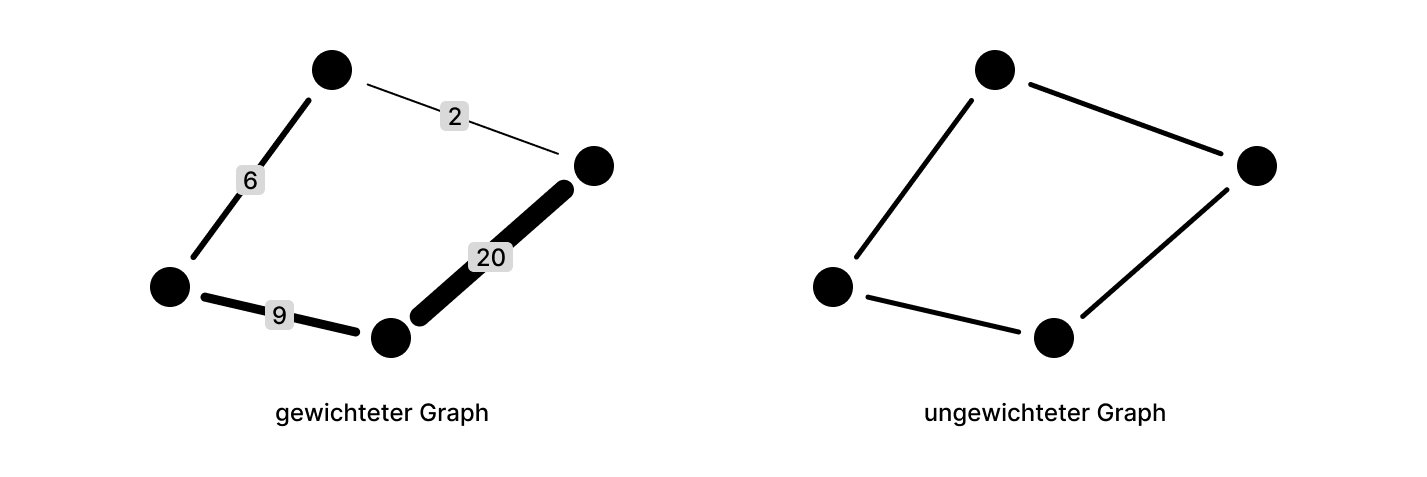
\includegraphics[width=1\textwidth]{content/img/Research/Graphen/Gewicht.png}
    \caption{Ein Graph, welcher gewichtete Kanten hat (links); ein Graph, dessen Kanten immer das gleiche Gewicht haben (rechts)}
    \label{fig:gewicht}
\end{figure}
\FloatBarrier